\documentclass[border=0pt]{standalone}
\usepackage[left=25mm,right=25mm,top=25mm,bottom=25mm]{geometry}
\usepackage[utf8]{inputenc}
\usepackage[T1]{fontenc}
\usepackage{times}
\usepackage{geometry}
\usepackage{amsmath}
\usepackage{amssymb}
\usepackage{mathrsfs}
\usepackage{amsfonts}
\usepackage{amsthm}
\usepackage{lipsum}
\usepackage{amscd}
\usepackage{graphicx}
\usepackage{fancyhdr}
\usepackage{textcomp}
\usepackage{txfonts}
\usepackage[all]{xy}
\usepackage{paralist}
\usepackage[colorlinks=true]{hyperref}
\usepackage{array}
\usepackage{tikz}
\usepackage{slashed}
\usepackage{pdfpages}
\usepackage{cite}
\usepackage{url}

\usepackage{listings}
\usepackage{multirow}
\usepackage{color}

\begin{document}



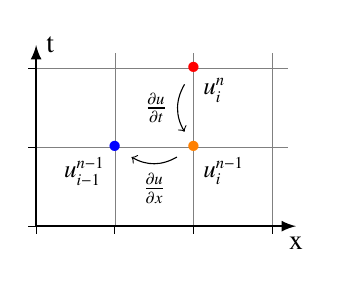
\begin{tikzpicture}
  \draw[thick,step=1cm,help lines] (0,0) grid (3.2,2.2);
  %\draw[ultra thin,step=.5cm,help lines] (0,0) grid (5,5);
  % Draw axes
  \draw[thick,-latex] (0,0) -- (3.3,0) node[anchor=north](){x};
  \draw[thick,-latex] (0,0) -- (0,2.3) node[anchor= west](){t};
  % the co-ordinates -- major
  \foreach \x in {0,1,...,3}  {   % for x-axis
  \draw [] (\x,0) -- (\x,-0.1);
  }
  \foreach \y in {0,1,...,2} {   %% for y-axis
  \draw [] (0,\y) -- (-0.1,\y);
  }
  % the numbers
  % \foreach \x in {0,1,...,3} { \node [anchor=center] at (\x,0.2) {\tiny \x}; }
  % \foreach \y in {0,1,...,3} { \node [anchor=center] at (-0.2,-\y) {\tiny \y}; }

  \draw (2,2) node[red, anchor=center](1){\textbullet};
  \draw (2,2) node[anchor=north west]{\small$u_{i}^{n}$};
  \draw (2,1) node[orange, anchor=center](3){\textbullet};
  \draw (2,1) node[anchor=north west]{\small$u_{i}^{n-1}$};
  \draw (1,1) node[blue, anchor=center](4){\textbullet};
  \draw (1,1) node[anchor=north east]{\small$u_{i-1}^{n-1}$};
  \draw [->] (3) to [out=210,in=-30]node[anchor=north]{\small $\frac{\partial u}{\partial x}$} (4);
  \draw [->] (1) to [out=240,in=120]node[anchor=east]{\small $\frac{\partial u}{\partial t}$} (3);


\end{tikzpicture}


\end{document}
